\documentclass{standalone}
\usepackage{tikz}

\begin{document}
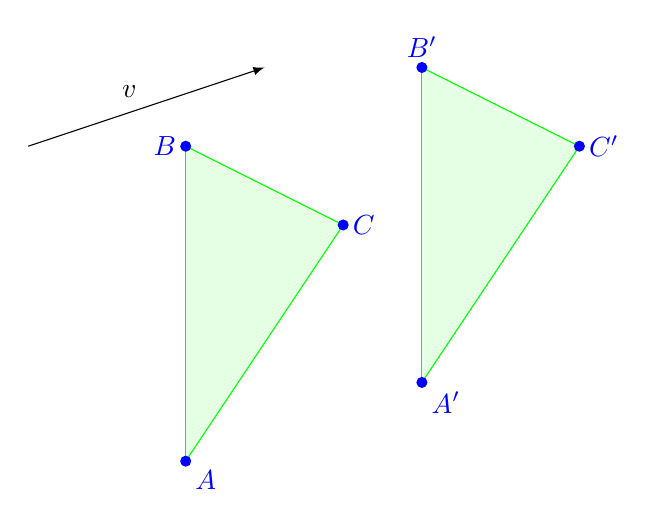
\begin{tikzpicture}[>=latex,scale=2]
\fill[color=green,fill=green,fill opacity=0.1] (0,0) -- (0,2) -- (1,1.5) -- cycle;
\fill[color=green,fill=green,fill opacity=0.1] (1.5,2.5) -- (1.5,0.5) -- (2.5,2) -- cycle;
\draw [color=green] (0,0)-- (0,2);
\draw [color=green] (0,2)-- (1,1.5);
\draw [color=green] (1,1.5)-- (0,0);
% \draw [->] (0,2) -- (1.5,2.5);
\draw [color=green] (1.5,2.5)-- (1.5,0.5);
\draw [color=green] (1.5,0.5)-- (2.5,2);
\draw [color=green] (2.5,2)-- (1.5,2.5);
\draw [->] (-1,2) --node[above left]{$v$} (0.5,2.5);
\fill [color=blue] (0,0) circle (1pt) node [below right] {$A$};
\fill [color=blue] (0,2) circle (1pt) node [left] {$B$};
\fill [color=blue] (1,1.5) circle (1pt) node [right] {$C$};
\fill [color=blue] (1.5,2.5) circle (1pt) node [above] {$B'$};
\fill [color=blue] (2.5,2) circle (1pt) node [right] {$C'$};
\fill [color=blue] (1.5,0.5) circle (1pt) node [below right] {$A'$};
% \fill [color=blue] (-1,2) node [above left] {$E$};
% \fill [color=blue] (0.5,2.5) node [above] {$E'$};
\end{tikzpicture}
\end{document}